\documentclass[a4paper,12pt]{article}

\usepackage[utf8]{inputenc}
\usepackage[T1]{fontenc}
\usepackage{amsmath}
\usepackage{booktabs}
\usepackage{graphicx}
\usepackage{geometry}
\geometry{margin=2.5cm}
\usepackage{xcolor}
\usepackage{listings}
\usepackage{hyperref}
\usepackage{float}
\hypersetup{colorlinks=true, linkcolor=blue!50!black, urlcolor=blue!50!black}
\renewcommand{\tablename}{Tabela}
\renewcommand{\figurename}{Figura}
\renewcommand{\lstlistingname}{Código}

% ---------- Configuração do realce de sintaxe (C) ----------
\definecolor{codebg}{RGB}{247,247,247}
\definecolor{codekw}{RGB}{0,0,180}
\definecolor{codecomment}{RGB}{0,128,0}
\definecolor{codestring}{RGB}{163,21,21}
\definecolor{framecolor}{RGB}{200,200,200}

\lstdefinestyle{cstyle}{
    language=C,
    backgroundcolor=\color{codebg},
    basicstyle=\ttfamily\footnotesize,
    keywordstyle=\color{codekw}\bfseries,
    commentstyle=\color{codecomment}\itshape,
    stringstyle=\color{codestring},
    numberstyle=\tiny\color{gray},
    numbers=left,
    numbersep=6pt,
    frame=single,
    rulecolor=\color{framecolor},
    breaklines=true,
    breakatwhitespace=false,
    showstringspaces=false,
    tabsize=4,
    captionpos=b,
    columns=flexible,
    morekeywords={size_t},
    extendedchars=true,
    literate=
        {á}{{\'a}}1 {à}{{\`a}}1 {â}{{\^a}}1 {ã}{{\~a}}1
        {é}{{\'e}}1 {ê}{{\^e}}1 {í}{{\'i}}1
        {ó}{{\'o}}1 {ô}{{\^o}}1 {õ}{{\~o}}1
        {ú}{{\'u}}1 {ü}{{\"u}}1 {ç}{{\c c}}1
        {Á}{{\'A}}1 {À}{{\`A}}1 {Â}{{\^A}}1 {Ã}{{\~A}}1
        {É}{{\'E}}1 {Ê}{{\^E}}1 {Í}{{\'I}}1
        {Ó}{{\'O}}1 {Ô}{{\^O}}1 {Õ}{{\~O}}1
        {Ú}{{\'U}}1 {Ü}{{\"U}}1 {Ç}{{\c C}}1
        {ª}{{\textordfeminine}}1 {º}{{\textordmasculine}}1
}

\title{Tarefa 15: Sobreposição de Computação e Comunicação}
\author{Israel Soares de Castro Filho \\ Matrícula: 20250070780}
\date{}

\begin{document}

\maketitle

\section{Introdução}

O objetivo desta tarefa é medir quanto se ganha ao sobrepor comunicação e
computação em um programa MPI. O problema escolhido é a difusão de calor em
uma barra 1D dobrada em anel (contorno periódico), resolvida por diferenças
finitas explícitas. A barra é dividida entre os processos, e a cada passo de
tempo vizinhos precisam trocar suas células de borda.

Foram implementadas três versões da troca de bordas:
\begin{itemize}
    \item \textbf{V1:} \texttt{MPI\_Send} / \texttt{MPI\_Recv} (bloqueante);
    \item \textbf{V2:} \texttt{MPI\_Isend} / \texttt{MPI\_Irecv} e \texttt{MPI\_Wait};
    \item \textbf{V3:} igual à V2, mas calculando os pontos internos enquanto
          a comunicação acontece, com \texttt{MPI\_Test}.
\end{itemize}

Ferramentas utilizadas: MPI e o supercomputador NPAD.

\section{Metodologia}

\paragraph{Decomposição e células fantasmas.}
Cada processo guarda um trecho contíguo da barra, com $n$ células reais mais
duas células fantasmas (\emph{ghost cells}): $u[0]$ recebe a última célula
real do vizinho da esquerda e $u[n+1]$ recebe a primeira célula real do
vizinho da direita. Como a barra é um anel, o processo 0 é vizinho do último
processo. Duas tags distinguem o sentido das mensagens (direita e esquerda),
o que também funciona com apenas 2 processos.

\paragraph{As três versões.}
\begin{itemize}
    \item \textbf{V1:} a troca é feita em duas fases em cadeia (primeiro
          para a direita, depois para a esquerda). O processo 0 envia
          primeiro para quebrar o ciclo e evitar \emph{deadlock}; os demais
          recebem primeiro e depois enviam.
    \item \textbf{V2:} os quatro \texttt{Isend}/\texttt{Irecv} são postados
          de uma vez, o programa espera todos com \texttt{MPI\_Wait} e só
          então calcula todas as células.
    \item \textbf{V3:} após postar as operações, calcula os pontos internos
          (que não dependem do halo) em blocos de 100 células, chamando
          \texttt{MPI\_Test} entre os blocos. Depois espera o fim da
          comunicação e calcula as duas células de borda.
\end{itemize}

\paragraph{Experimentos.}
Os testes rodaram no NPAD com 2 nós, com 2, 4 e 8 processos distribuídos
entre eles (1, 2 e 4 processos por nó), e com $N = 1000$, $5000$ e $10000$
pontos. O tempo de cada versão foi medido com \texttt{MPI\_Wtime} e
corresponde ao maior tempo entre os processos, contando só cálculo e
comunicação.

\section{Resultados}

A Figura~\ref{fig:barras} mostra a evolução da temperatura obtida pelas
três versões. Os resultados são visualmente idênticos, o que indica que a
troca de células fantasmas está correta em todas elas: o calor se espalha a
partir do centro e a barra tende ao equilíbrio.

\begin{figure}[h]
    \centering
    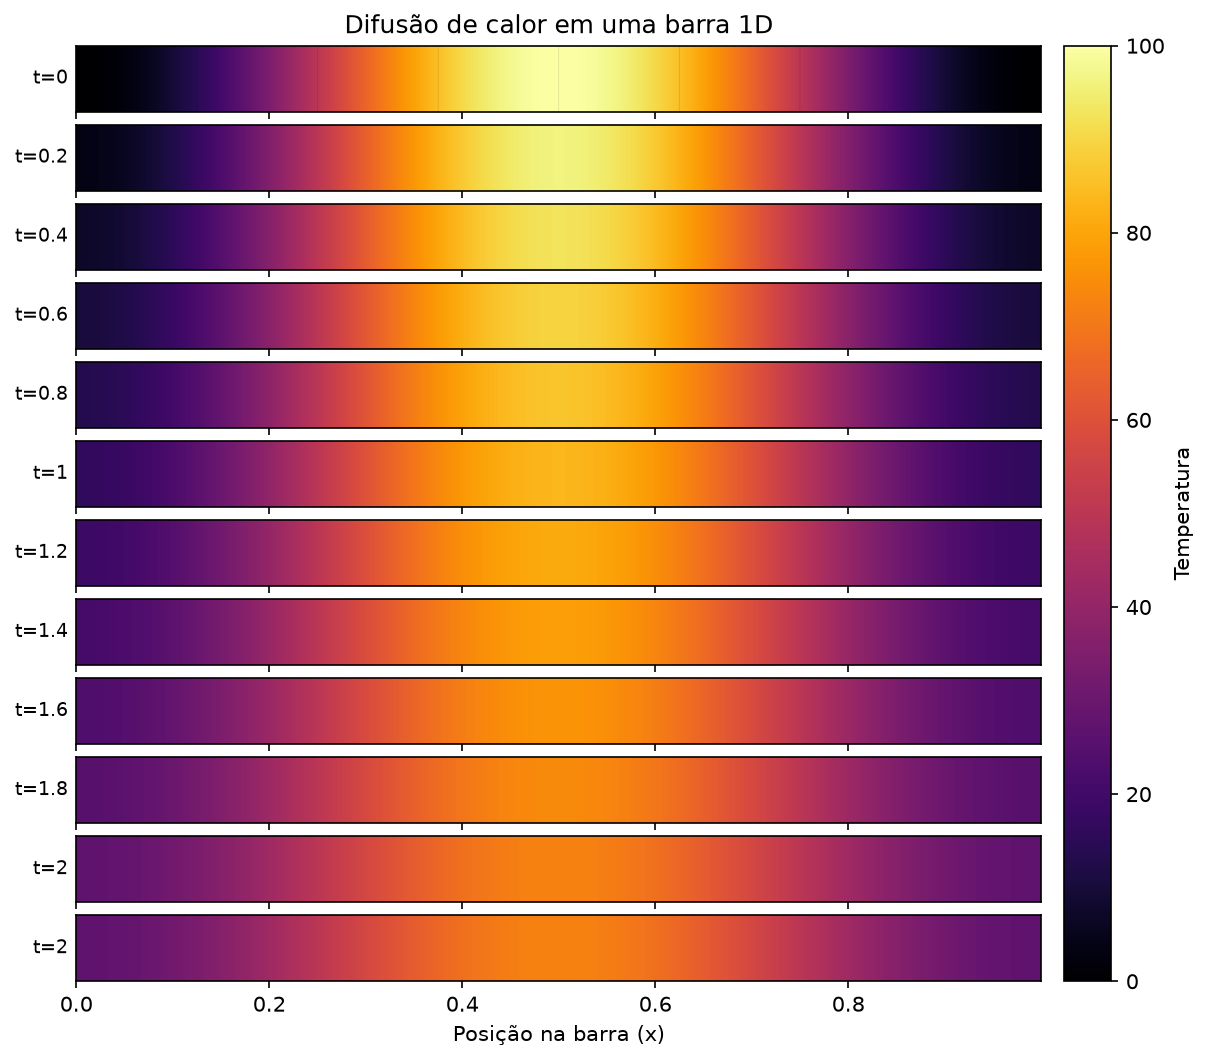
\includegraphics[width=0.32\textwidth]{../images/barras/versao1.png}
    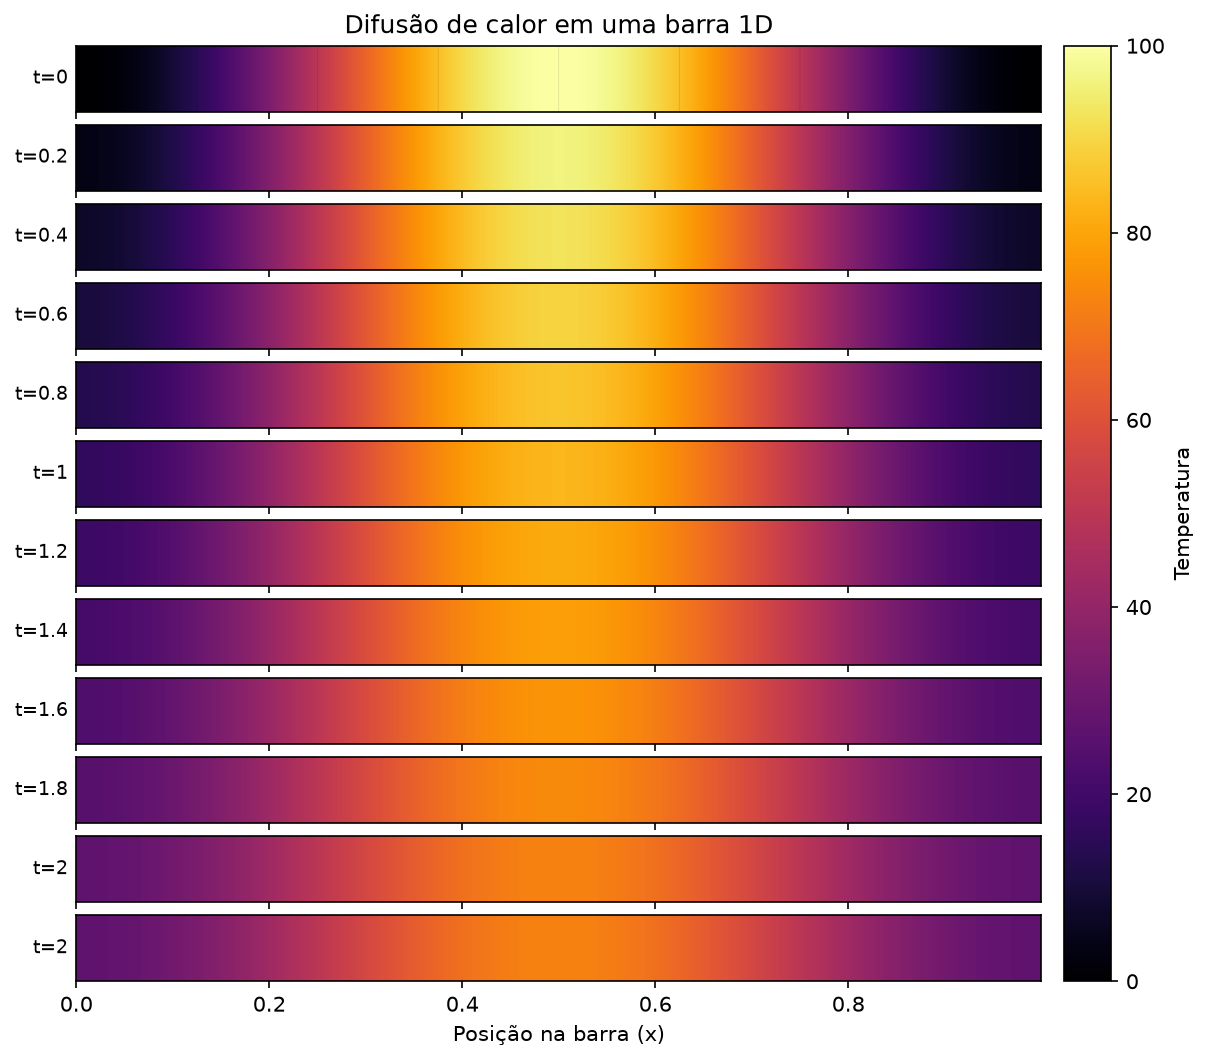
\includegraphics[width=0.32\textwidth]{../images/barras/versao2.png}
    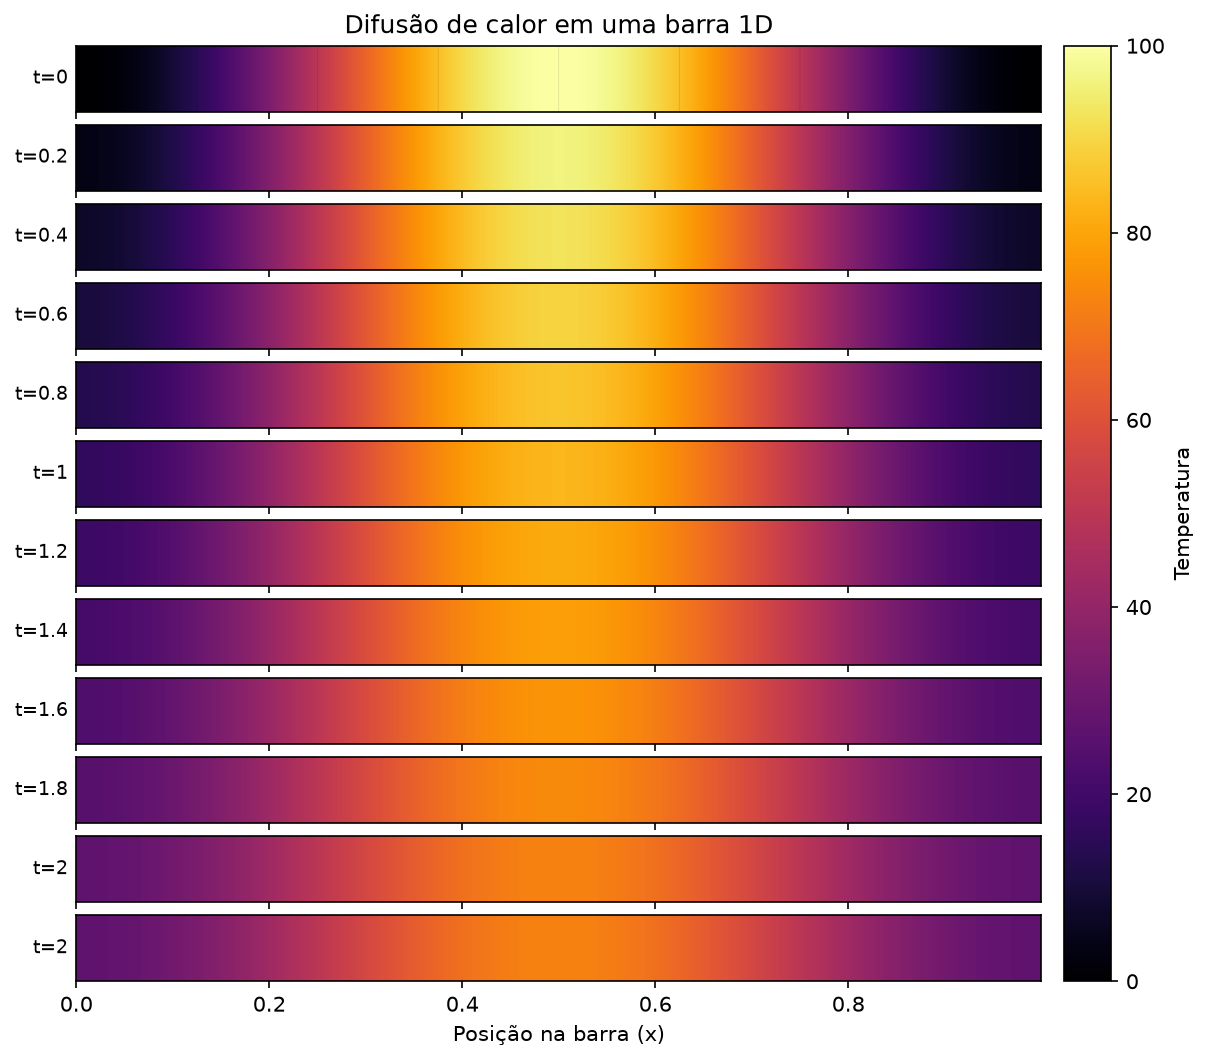
\includegraphics[width=0.32\textwidth]{../images/barras/versao3.png}
    \caption{Evolução da temperatura na barra: V1, V2 e V3 (da esquerda para a direita).}
    \label{fig:barras}
\end{figure}

A Tabela~\ref{tab:tempos} reúne os tempos medidos e o ganho de V2 e V3 em
relação à V1.

\begin{table}[h]
    \centering
    \begin{tabular}{rrrrrrr}
        \toprule
        $N$ & Proc. & V1 (s) & V2 (s) & V3 (s) & V1/V2 & V1/V3 \\
        \midrule
        1000  & 2 & 0,205 & 0,143 & 0,136 & 1,43 & 1,50 \\
        1000  & 4 & 0,319 & 0,127 & 0,103 & 2,51 & 3,10 \\
        1000  & 8 & 0,626 & 0,145 & 0,118 & 4,31 & 5,29 \\
        \midrule
        5000  & 2 & 11,71 & 10,13 & 12,52 & 1,16 & 0,94 \\
        5000  & 4 & 10,91 & 6,26  & 7,24  & 1,74 & 1,51 \\
        5000  & 8 & 18,13 & 5,90  & 6,41  & 3,07 & 2,83 \\
        \midrule
        10000 & 2 & 80,42 & 73,95 & 96,59 & 1,09 & 0,83 \\
        10000 & 4 & 60,50 & 40,93 & 51,07 & 1,48 & 1,18 \\
        10000 & 8 & 88,25 & 39,47 & 44,66 & 2,24 & 1,98 \\
        \bottomrule
    \end{tabular}
    \caption{Tempos de execução e ganho sobre a V1 (valores acima de 1 indicam que a versão é mais rápida que a V1).}
    \label{tab:tempos}
\end{table}

\begin{figure}[h]
    \centering
    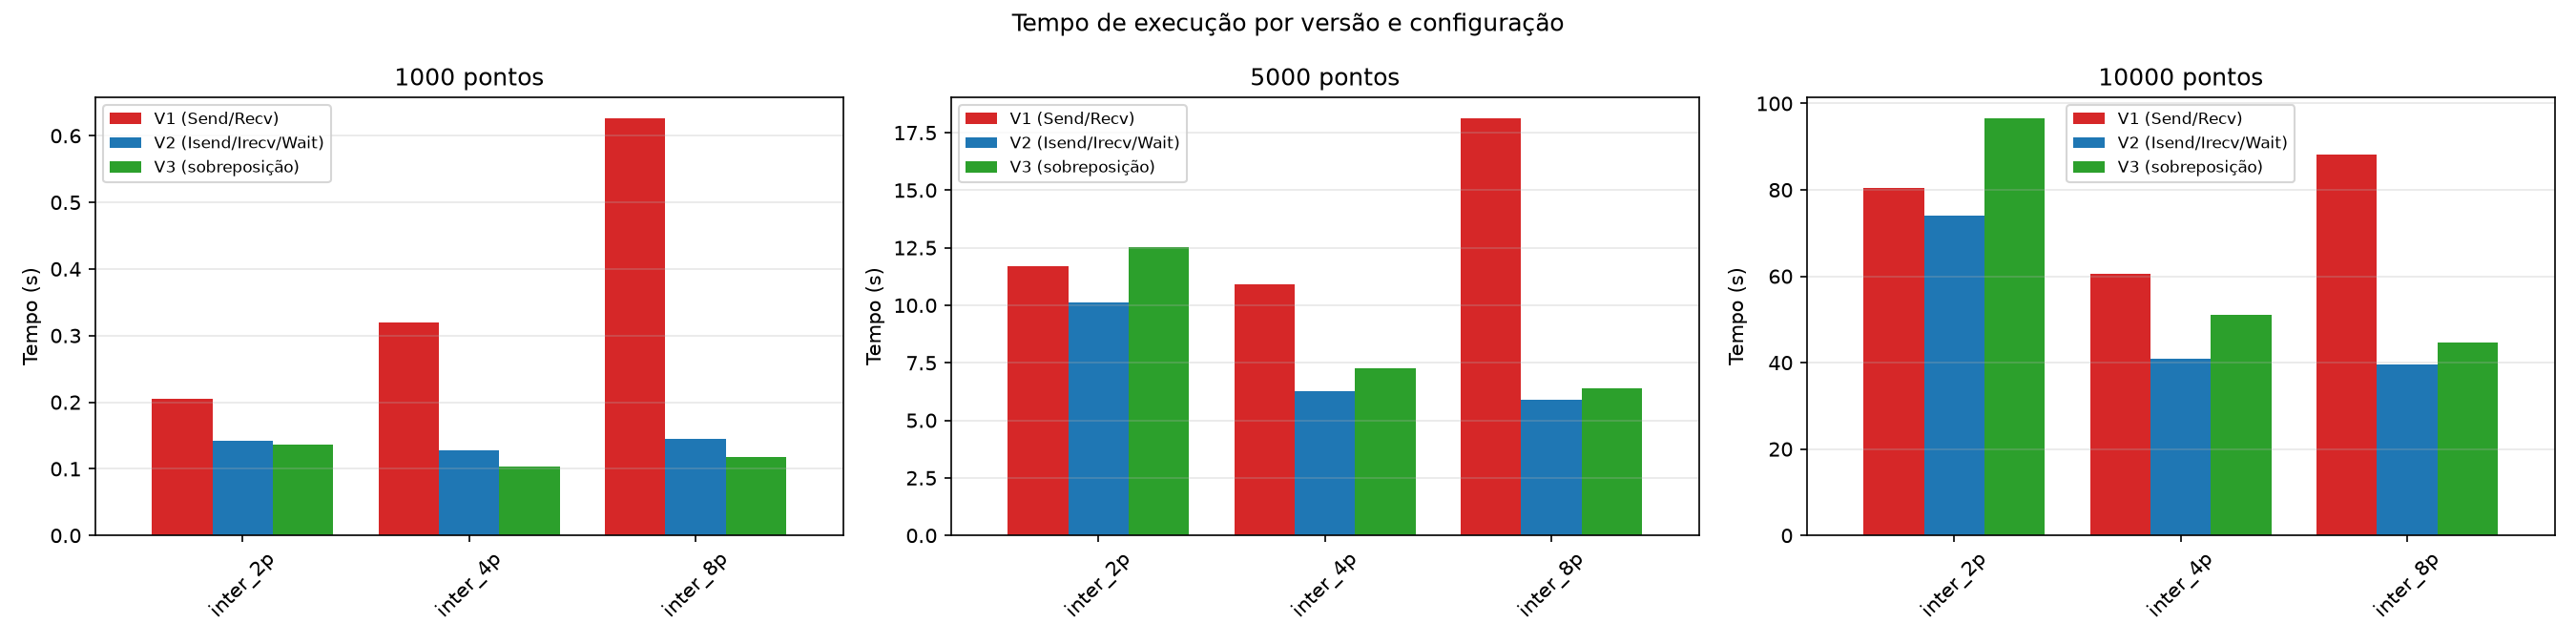
\includegraphics[width=\textwidth]{../images/graficos/tempos_barras.png}
    \caption{Tempo de execução de cada versão por configuração.}
    \label{fig:tempos}
\end{figure}

\begin{figure}[h]
    \centering
    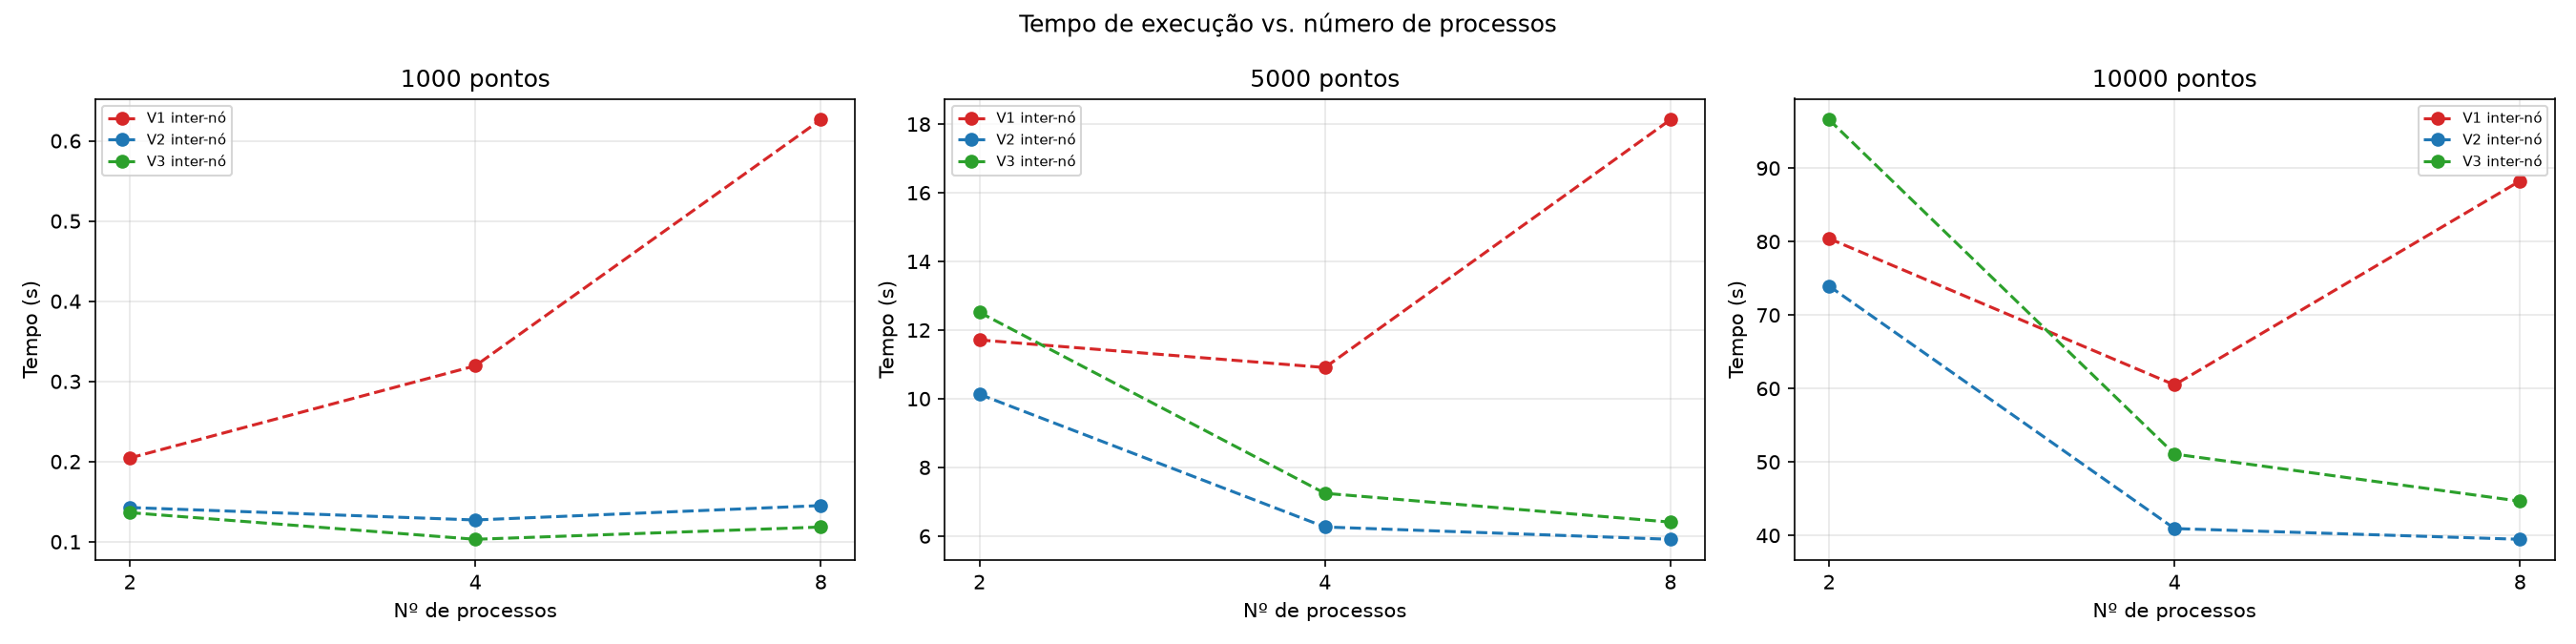
\includegraphics[width=\textwidth]{../images/graficos/escalabilidade.png}
    \caption{Tempo de execução em função do número de processos.}
    \label{fig:escala}
\end{figure}

\begin{figure}[h]
    \centering
    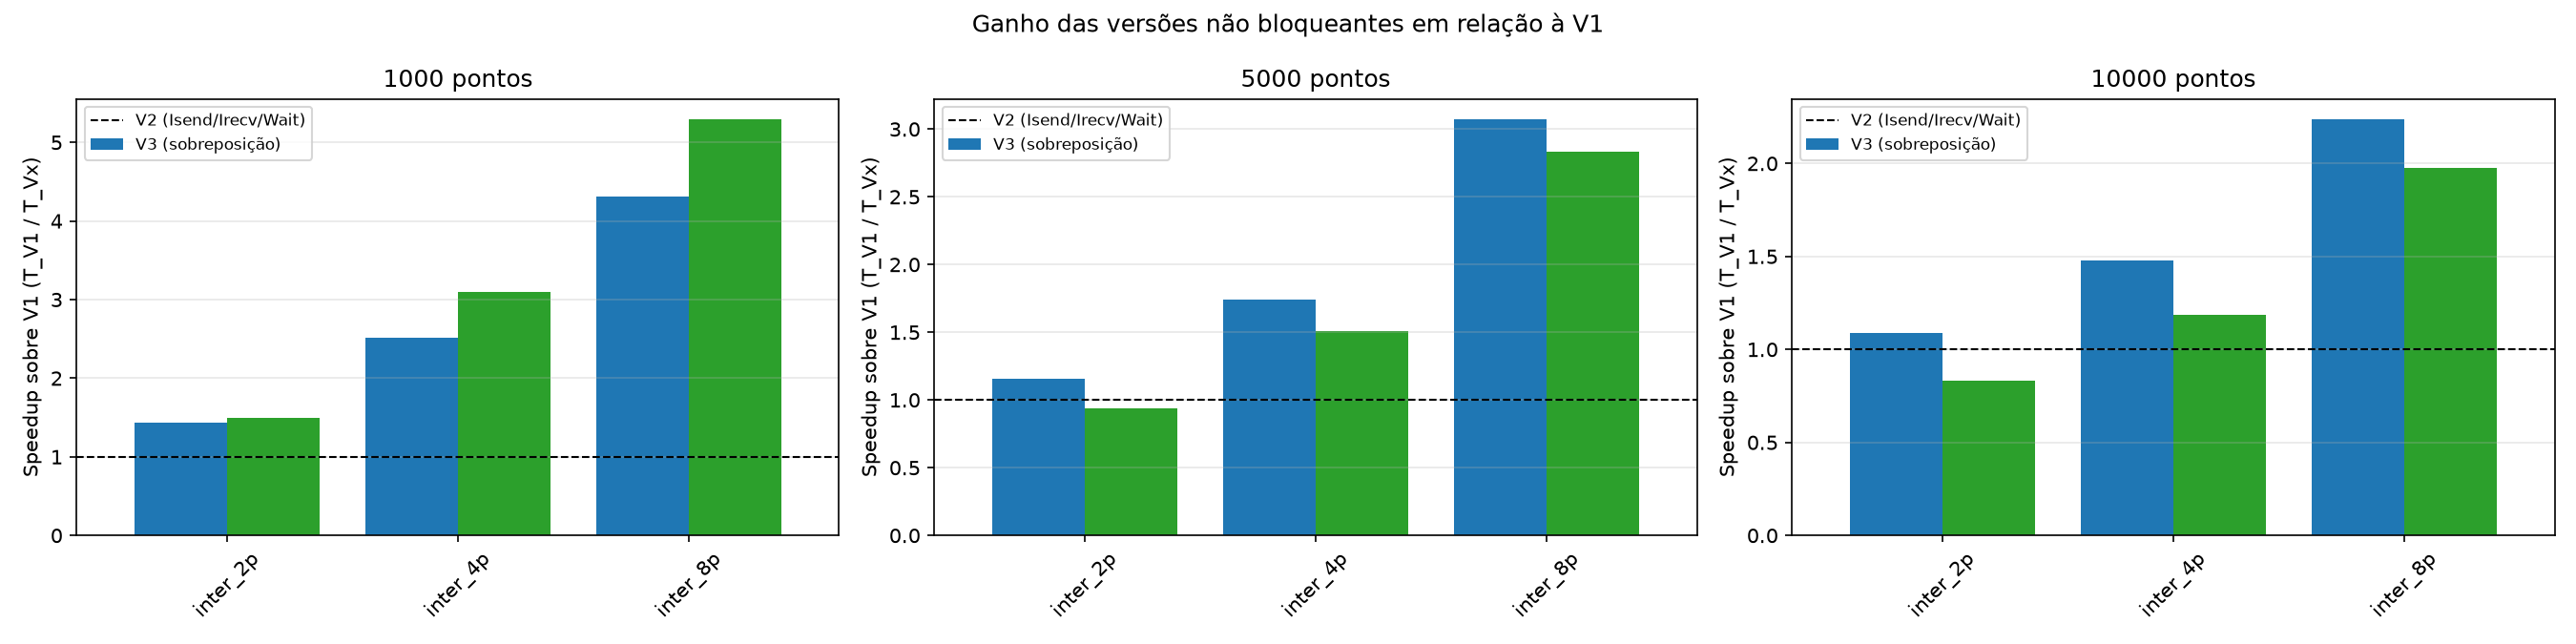
\includegraphics[width=\textwidth]{../images/graficos/speedup_vs_v1.png}
    \caption{Ganho de V2 (azul) e V3 (verde) em relação à V1.}
    \label{fig:speedup}
\end{figure}

\section{Análise}

\paragraph{Impacto das versões no tempo.}
A escolha da versão muda bastante o tempo de execução. Para $N=1000$ e 8
processos, a V1 leva 0,63~s contra 0,15~s da V2 e 0,12~s da V3. Com 8
processos, V2 e V3 foram de 2 a 5 vezes mais rápidas que a V1 em todos os
tamanhos testados.

\paragraph{A V1 piora com mais processos.}
Mesmo com $N$ fixo, o tempo da V1 tende a crescer quando se aumentam os
processos (Figura~\ref{fig:escala}). Com $N=1000$, ele sobe de 0,20~s para
0,63~s ao passar de 2 para 8 processos, embora cada processo tenha menos
células para calcular. A causa é o bloqueio: na V1 cada processo só envia
depois de receber do anterior, então a troca de bordas vira uma cadeia e o
tempo de comunicação cresce com o número de processos, enquanto os demais
ficam esperando. Nos tamanhos maiores o efeito é mascarado pelo cálculo, mas
continua visível (por exemplo, $N=10000$ passa de 60,5~s com 4 processos para
88,3~s com 8).

\paragraph{Impacto da V2 e da V3.}
Na V2 as quatro operações são postadas ao mesmo tempo, então as trocas de
todos os pares acontecem em paralelo e o custo de comunicação deixa de
crescer com o número de processos. Com $N=1000$ o tempo fica praticamente
constante (0,13 a 0,15~s), e com $N$ maior ele cai conforme se adicionam
processos. Já a V3 teve comportamento misto em relação à V2, discutido a
seguir.

\paragraph{Ganho com a sobreposição.}
Para $N=1000$, a sobreposição compensou: a V3 foi cerca de 19\% mais rápida
que a V2 com 4 e 8 processos (e 4\% com 2), e é onde a comunicação pesa mais
no tempo total. Para $N=5000$ e $N=10000$, porém, a V3 ficou mais lenta que
a V2 (até 31\% mais lenta, em $N=10000$ com 2 processos). 

Uma explicação
provável é o custo das chamadas de \texttt{MPI\_Test}: com blocos de 100
células, são 4 chamadas por bloco a cada passo, e esse número cresce com o
tamanho do trecho de cada processo. Ou seja, a sobreposição só vale a
pena quando o que ela esconde é maior que o custo de testar a comunicação, e
o tamanho do bloco é o parâmetro que controla esse equilíbrio.

\paragraph{Limitações.}
Cada configuração foi medida uma só vez, então diferenças pequenas (como
V3 contra V1 em $N=5000$ com 2 processos) podem ser ruído. Os testes
registraram avisos do Open MPI sobre a placa InfiniBand, e a comunicação
entre nós pode ter usado um caminho mais lento que o ideal, o que também
afeta os tempos absolutos.

\section{Conclusão}

\begin{itemize}
    \item A troca bloqueante da V1 não escala: seu tempo cresce com o número
          de processos mesmo para $N$ fixo, por causa da espera em cadeia.
    \item Comunicação não bloqueante (V2) resolve esse problema e foi, no
          geral, a versão mais regular, com ganhos de até 4,3 vezes sobre a V1.
    \item A sobreposição com \texttt{MPI\_Test} (V3) trouxe o melhor tempo
          nos casos pequenos ($N=1000$), mas perdeu para a V2 nos maiores,
          mostrando que o ganho depende de ajustar a frequência dos testes.
    \item Como continuação, vale testar blocos maiores (ou menos chamadas de
          \texttt{MPI\_Test}) na V3 e repetir as medições para obter médias.
\end{itemize}

\newpage
\appendix

\section{Código-Fonte}

\lstinputlisting[style=cstyle, caption={Simulação da barra 1D em anel com MPI (V1, V2 e V3).}, label={cod:mpi}]{../src/tarefa15.c}

\end{document}